\documentclass{standalone}
\usepackage{xparse}
\usepackage{tikz}
\usepackage{graphicx}
\usetikzlibrary{shapes}

\newdimen\hexdim % goes into the preamble
\hexdim=1cm

\ExplSyntaxOn
\DeclareExpandableDocumentCommand{\getlengthratio}{mm}
 {
  \fp_eval:n { floor ( \dim_to_fp:n { #1 } / \dim_to_fp:n { #2 } , 0 ) }
 }
\ExplSyntaxOff

\newcount\xhexes
\xhexes=\getlengthratio{\textwidth}{\hexdim}

\newdimen\imageheight % goes into the preamble

\settoheight{\imageheight}{%
  \includegraphics[width=\textwidth,keepaspectratio]{example-image}%
}

\newcount\yhexes
\yhexes=\getlengthratio{\imageheight}{\hexdim}

\begin{document}
  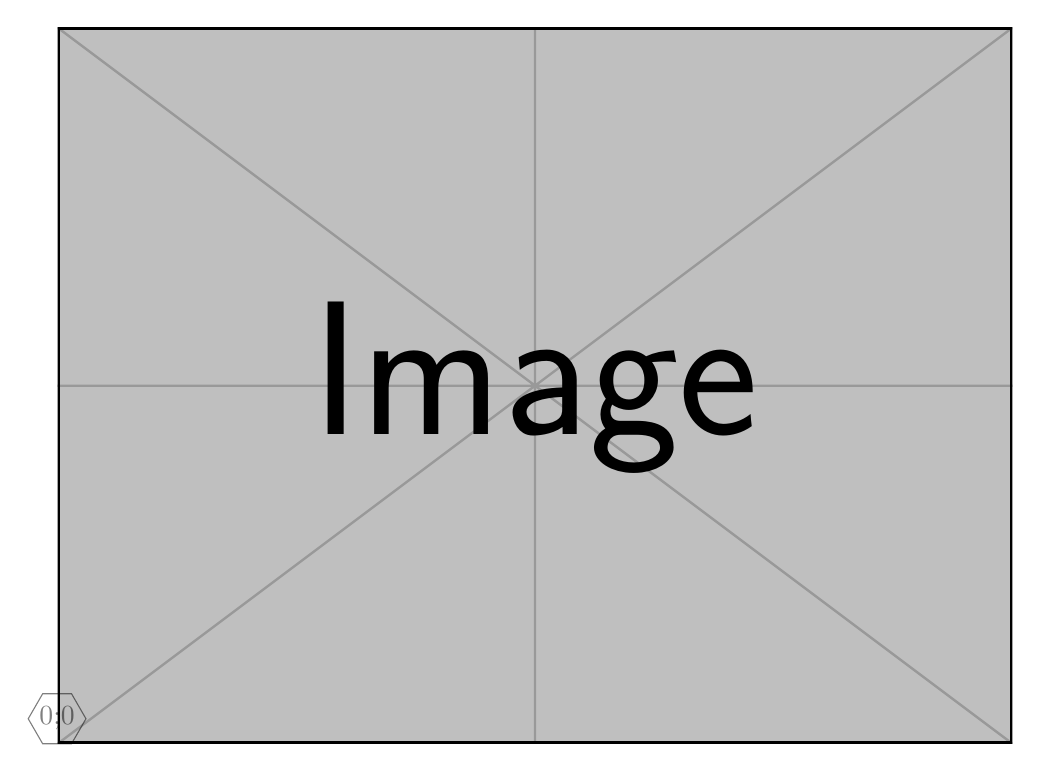
\begin{tikzpicture} [hexa/.style= {shape=regular polygon,
                                     regular polygon sides=6,
                                     minimum size=\hexdim, draw,
                                     inner sep=0,anchor=south,
                                     opacity=.5}]

      \node[anchor=south west,inner sep=0] (image) at (0,0) {\includegraphics[width=\textwidth]{example-image}};
      \foreach \j in {0,...,\xhexes}{% 
           \ifodd\j 
               \foreach \i in {0,...,\yhexes}{\node[hexa] (h\j;\i) at ({\j*\hexdim/2+\j*\hexdim/4+\hexdim/2},{(\i*\hexdim+\hexdim/2)*sin(60)}) {\j;\i};}        
          \else
               \foreach \i in {0,...,\yhexes}{\node[hexa] (h\j;\i) at ({\j*\hexdim/2+\j*\hexdim/4+\hexdim/2},{\i*\hexdim*sin(60)}) {\j;\i};}
          \fi}
  \end{tikzpicture}

\the\hexdim
\the\imageheight
\the\yhexes
\end{document}      
